% !TEX root = thesis.tex

\section{Source-level Debugging of Optimized Code}
\label{se:CS-debug}
A {\em source-level} (or {\em symbolic}) {\em debugger} is a program development tool that allows a programmer to monitor an executing program at the source-language level. Interactive mechanisms are typically provided to the user to halt/resume the execution at {\em breakpoints}, and to inspect the state of the program in terms of its source language.

The importance of the design and use of these tools was already clear in the '60s~\cite{Evans66}. In a production environment it is desirable to use optimizations, and bugs can surface when optimizations are enabled, as the debuggable translation of a program may hide them, or because differences in timing behavior may cause the appearance of bugs due to race conditions~\cite{Adl-Tabatabai96thesis}. Also, optimizations may be absolutely necessary to execute a program: for example, because of memory limitations, efficiency reasons, or other platform-specific constraints.

As pointed out by Hennessy in his '82 seminal paper~\cite{Hennessy82}, a classic conflict exists between the application of optimization techniques and the ability to debug a program symbolically. A debugger provides the user with the illusion that the source program is executing one statement at a time. On the other hand, optimizations preserve the semantic equivalence between optimized and unoptimized code, but normally alter the structure and the intermediate results of a program.

Two problems surface when trying to symbolically debug optimized code~\cite{Adl-Tabatabai96,Jaramillo00}. First, the debugger must determine the position in the optimized code that corresponds to the breakpoint in the source code ({\em code location} problem). Second, the user expects to see the values of source variables at a breakpoint in a manner consistent with the source code, even though the optimizer might have 
deleted or reordered instructions, or values might have been overwritten as a consequence of register allocation choices ({\em data location} problem).

\noindent When attempting to debug optimized programs, debuggers may thus give misleading information about the value of variables at breakpoints. Hence, the programmer has the difficult task of attempting to unravel the optimized code and determine what values the variables should have~\cite{Hennessy82}.

In general, there are two ways for a symbolic debugger to present meaningful information about the debugged optimized program~\cite{Wu99}. It provides {\em expected behavior} of the program if it hides the effect of the optimizations from the user and presents the program state consistent with what they expect from the unoptimized code. It provides {\em truthful behavior} if it makes the user aware of the effects of optimizations and warns of possibly surprising outcomes.

In his PhD thesis Adl-Tabatabai observes that constraining optimizations or adding machinery during compilation to aid debugging do not solve the problem of debugging the optimized translation of a program, as the user debugs suboptimal code~\cite{Adl-Tabatabai96thesis}. Source-level debuggers thus need to implement techniques to recover expected behavior when possible, without relying on intrusive compiler extensions.

\subsection{Using \texorpdfstring{$\texttt{build\_comp}$}{build\_comp} for State Recovery}
%\subsection{Using  for State Recovery}
On-stack replacement has been pioneered in implementations of the SELF programming language to provide expected behavior with globally optimized code~\cite{Holzle92}. OSR shields the debugger from the effects of optimizations by dynamically deoptimizing code on demand. Debugging information is supplied by the compiler at discrete {\em interrupt points}, which act as a barrier for optimizations, letting the compiler run unhindered between them. Starting from the observation that our algorithms for generating OSR mappings (\mysection\ref{ss:osr-mapping}) do not place barriers for live-variable equivalent transformations, we investigated whether they can also encode useful information for expected-behavior recovery in a source-level debugger.

As in most recent works on optimized code debugging, we focus on identifying and recovering scalar source variables in the presence of global optimizations. In LLVM, debugging information is inserted by the front-end as {\em metadata} attached to global variables, single instructions, functions or entire IR modules.

Debugging metadata are transparent to optimization passes, do not prevent optimizations from happening, and are designed to be agnostic about both the source language in which the original program is written and the target debugging information representation (e.g., DWARF, stabs). Two intrinsics are used to associate IR virtual registers with source-level variables:
\begin{itemize}[itemsep=0pt,parsep=3pt]
 \item \mytt{llvm.dbg.declare} typically associates a source variable with an \alloca\footnote{\alloca\ is used to allocate space on the stack of the current function to be automatically released when the function returns. Front-ends are not required to generate code in SSA form, but they can manipulate local variables created with \alloca\ using \load\ and \store\ instruction. Then the SSA form can be constructed using \memtoreg.} buffer;
 \item \mytt{llvm.dbg.value} informs that a source variable is being set to the value held by the virtual register.
\end{itemize}

\noindent We extended \tinyvm\ to reconstruct this mapping and also to identify which program locations in the unoptimized IR version $f_{base}$ correspond to source-level locations for a function, which can become user breakpoints. An OSR mapping is then generated when OSR-aware transformation passes are applied to $f_{base}$ to generate the optimized version $f_{opt}$. For each location in $f_{opt}$ that might correspond to (i.e., have as OSR landing pad) a source-level location in $f_{base}$, we determine which variables live at the destination are live also at the source (and thus they yield the same value), and which instead need to be reconstructed. We rely on the SSA form to identify which assignment(s) should be recovered by \reconstruct, as every value instance for a source-level variable is represented by a specific virtual register. $\phi$-nodes at control-flow merge points can not be reconstructed, but our experimental results suggest that this might not be a frequent issue in practice.

%As pointed out in~\cite{Adl-Tabatabai96}, compiler transformations cause {\em endangered} variables by either eliminating or moving assignments to source variables. 

\subsection{The \texorpdfstring{$\texttt{SPEC CPU2006}$}{SPEC CPU2006} Benchmarks}

\begin{table}[!t]
\begin{center}
\begin{small}
\begin{tabular}{ |c|r|r|r|r|r|r|r| }
\cline{3-8}
\multicolumn{2}{l|}{} & \multicolumn{6}{c|}{Functions} \\
\cline{3-8}
\multicolumn{2}{l|}{} & \multicolumn{1}{c|}{Total} & \multicolumn{2}{c|}{Optimized} & \multicolumn{3}{c|}{Endangered} \\
\hline
Benchmark & \multicolumn{1}{c|}{LOC} & \multicolumn{1}{c|}{$|F_{tot}|$} & \multicolumn{1}{c|}{$|F_{opt}|$}  & \multicolumn{1}{c|}{\tiny$\frac{|F_{opt}|}{|F_{tot}|}$} & \multicolumn{1}{c|}{$|F_{end}|$} & \multicolumn{1}{c|}{\tiny$\frac{|F_{end}|}{|F_{tot}|}$} & \multicolumn{1}{c|}{\tiny$\frac{|F_{end}|}{|F_{opt}|}$} \\ 
\hline
\hline
bzip2 & 8\,293 & 100 & 66 & 0.66 & 24 & 0.24 & 0.36 \\ 
\hline
gcc & 521\,078 & 5\,577 & 3\,884 & 0.70 & 1\,149 & 0.21 & 0.30 \\
\hline
gobmk & 197\,215 & 2\,523 & 1\,664 & 0.66 & 893 & 0.35 & 0.54 \\ 
\hline
h264ref & 51\,578 & 590 & 466 & 0.79 & 163 & 0.28 & 0.35 \\ 
\hline
hmmer & 35\,992 & 538 & 429 & 0.80 & 80 & 0.15 & 0.19 \\ 
\hline
lbm & 1\,155 & 19 & 17 & 0.89 & 2 & 0.11 & 0.12 \\ 
\hline
libquantum & 4\,358 & 115 & 85 & 0.74 & 9 & 0.08 & 0.11\\ 
\hline
mcf & 2\,658 & 24 & 21 & 0.88 & 11 & 0.46 & 0.52 \\ 
\hline
milc & 15\,042 & 235 & 157 & 0.67 & 34 & 0.14 & 0.22\\ 
\hline
perlbench & 155\,418 & 1\,870 & 1\,286 & 0.69 & 593 & 0.32 & 0.46 \\ 
\hline
sjeng & 13\,847 & 144 & 113 & 0.78 & 31 & 0.22 & 0.27 \\ 
\hline
sphinx3 & 25\,090 & 369 & 275 & 0.75 & 76 & 0.21 & 0.28 \\ 
\hline
\end{tabular} 
\end{small}
\end{center}
\caption{\label{tab:CS-debug-benchmarks} Characteristics of the C benchmarks from the \speccpu\ suite.} 
\end{table}

To capture a variety of programming patterns and styles from applications with different sizes, we have analyzed each method from each C benchmark in the \speccpu\ suite~\cite{Henning06}, applying the same sequence of OSR-aware optimization passes used in \mysection\ref{ss:bc-exp-setup} to the baseline IR version obtained with \clang\ \mytt{-O0} and post-processed with \memtoreg. \mytable\ref{tab:CS-debug-benchmarks} reports for each benchmark the code size, the total number of functions in it, the number of functions amenable to optimization and, in turn, how many optimized functions report ``endangered'' user variables from the source-level debugging perspective.

We observe that the fraction of functions that do not benefit from optimizations (i.e., $1-|F_{opt}|/F_{tot}|$) ranges from one tenth to one third of the total number of functions. For the optimized functions, the fraction of those that belong to $F_{end}$ - defined as the set of functions that require recovery of the expected behavior - ranges from $0.11$ (\mytt{libquantum}) to $0.54$ (\mytt{gobmk}).

\begin{table}[!ht]
\begin{center}
\begin{small}
\begin{tabular}{ |c|C{1.4cm}|C{1.4cm}|C{0.95cm}|C{0.95cm}|r| }
\cline{2-6}
\multicolumn{1}{l|}{} & \multicolumn{2}{c|}{Fraction of affected} & \multicolumn{3}{c|}{Endangered user vars} \\
\multicolumn{1}{l|}{} & \multicolumn{2}{c|}{program points} & \multicolumn{3}{c|}{per affected point} \\
\hline
Benchmark & $Avg_w$ & $Avg_u$ & $Avg$ & $\sigma$ & $Max$ \\ 
\hline
\hline
bzip2 & 0.17 & 0.12 & 1.22 & 0.55 & 5 \\
\hline
gcc & 0.25 & 0.22 & 1.13 & 0.31 & 14 \\
\hline
gobmk & 0.40 & 0.29 & 1.48 & 0.72 & 9 \\
\hline
h264ref & 0.45 & 0.55 & 1.69 & 1.23 & 14 \\
\hline
hmmer & 0.17 & 0.22 & 1.13 & 0.37 & 5 \\
\hline
lbm & 0.30 & 0.51 & 1.97 & 1.37 & 3 \\
\hline
libquantum & 0.13 & 0.10 & 1.06 & 0.17 & 2 \\
\hline
mcf & 0.35 & 0.32 & 1.00 & - & 1 \\
\hline
milc & 0.24 & 0.21 & 1.14 & 0.29 & 3 \\
\hline
perlbench & 0.37 & 0.35 & 1.16 & 0.36 & 8 \\
\hline
sjeng & 0.26 & 0.20 & 1.24 & 0.42 & 3 \\
\hline
sphinx3 & 0.29 & 0.31 & 1.19 & 0.44 & 6 \\
\hline
\hline
%Mean & 0.28 & 0.28 & 1.28 & 0.52 & 6.08 \\ % arithmetic
Mean & 0.26 & 0.25 & 1.26 & 0.47 & 6.08 \\
\hline
\end{tabular} 
\end{small}
\end{center}
\caption{\label{tab:CS-debug-affected-points} Fraction of program points with endangered user variables, and number of affected variables. The second and third column report weighted $Avg_g$ and unweighted $Avg_u$ average, respectively, of the fraction of such points for functions in $F_{end}$. We use the number of IR instructions in the unoptimized code as weight for computing $Avg_w$, and consider only IR program points corresponding to source-level locations. We then show mean, std deviation, and peak number of endangered variables at such points.} 
\end{table}

\mytable\ref{tab:CS-debug-affected-points} reports figures that we have collected for functions in $F_{end}$. We observe that, on average, at more than one in every four program points there is at least a user variable whose source-level value might not be reported correctly by a debugger. For most functions in the benchmarks, the average number of affected user variables at such points ranges between $1$ and $2$, although for some benchmarks we observe high peak values at specific points (e.g., $9$ for \mytt{gobmk} and $14$ for \mytt{gcc} and \mytt{h264ref}).

To investigate possible correlations between the size of a function and the number of user variables affected by source-level debugging issues, we analyzed the corpus of functions for the three largest benchmarks in our suite, namely \mytt{gcc}, \mytt{gobmk}, and \mytt{perlbench}. \myfigure\ref{fig:CS-debug-ratio} reports scatter plots in which each point represents a function: the horizontal position is given by the number of IR instructions in the unoptimized code, while the vertical position by the sum of the number of endangered user variables across program points corresponding to source-level locations.

\begin{figure}[!t]
\begin{center}
\centerline{
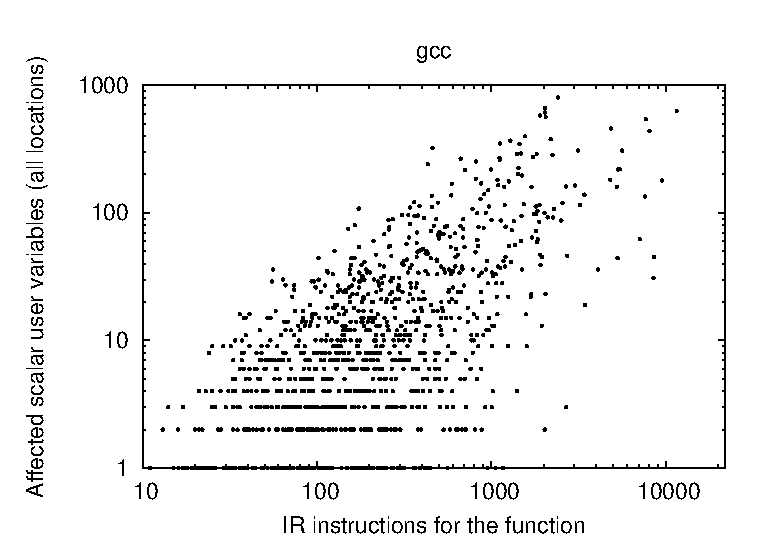
\includegraphics[width=0.45\textwidth]{figures/CS-debug-tot-dead/tot-dead-gcc-logscale.eps}
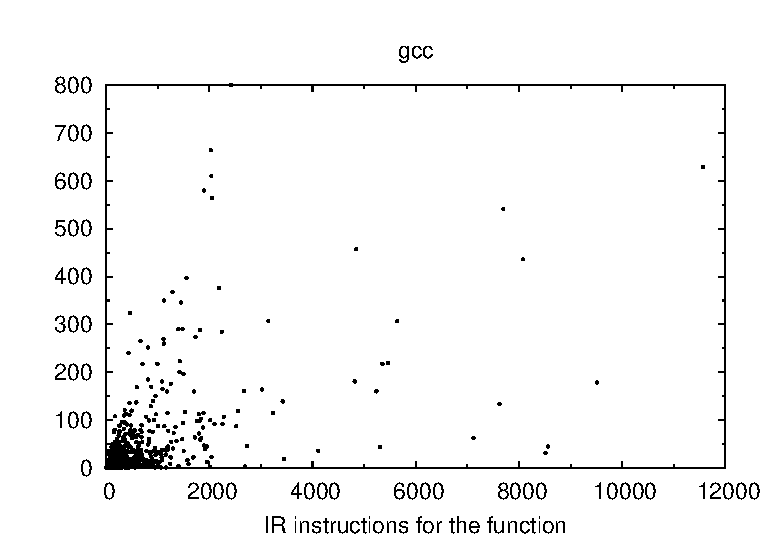
\includegraphics[width=0.45\textwidth]{figures/CS-debug-tot-dead/tot-dead-gcc-linear.eps}
}
\vspace{2mm}
\centerline{
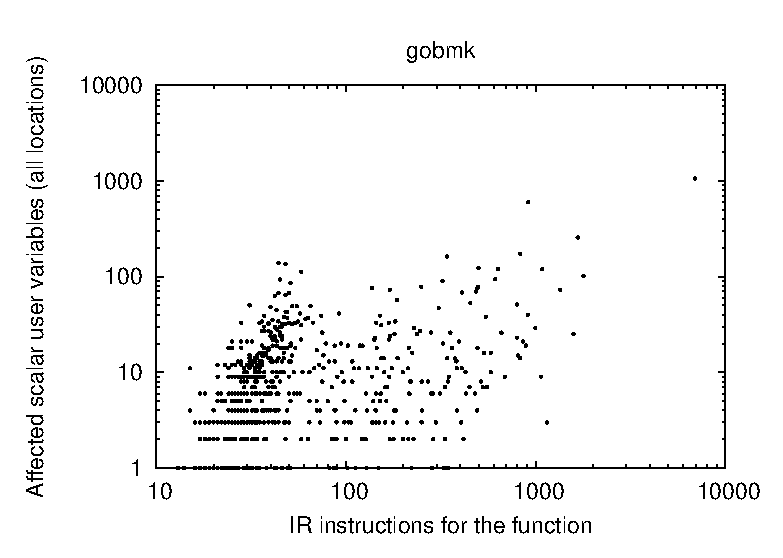
\includegraphics[width=0.45\textwidth]{figures/CS-debug-tot-dead/tot-dead-gobmk-logscale.eps}
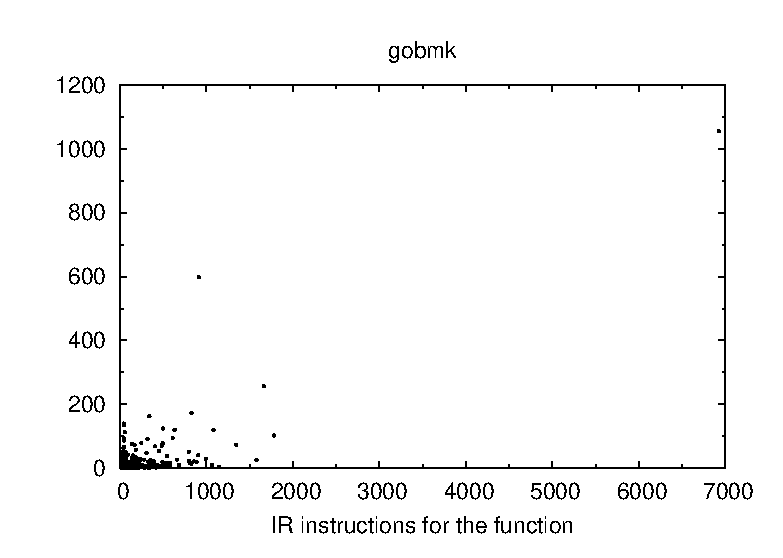
\includegraphics[width=0.45\textwidth]{figures/CS-debug-tot-dead/tot-dead-gobmk-linear.eps}
}
\vspace{2mm}
\centerline{
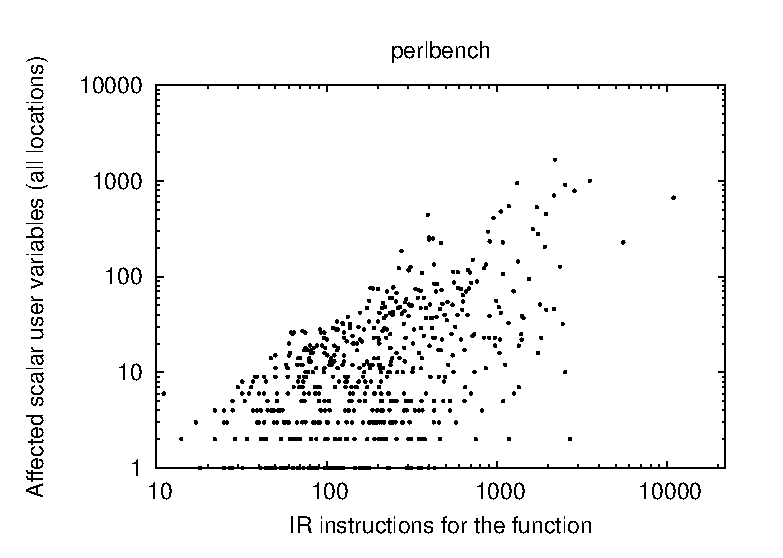
\includegraphics[width=0.45\textwidth]{figures/CS-debug-tot-dead/tot-dead-perlbench-logscale.eps}
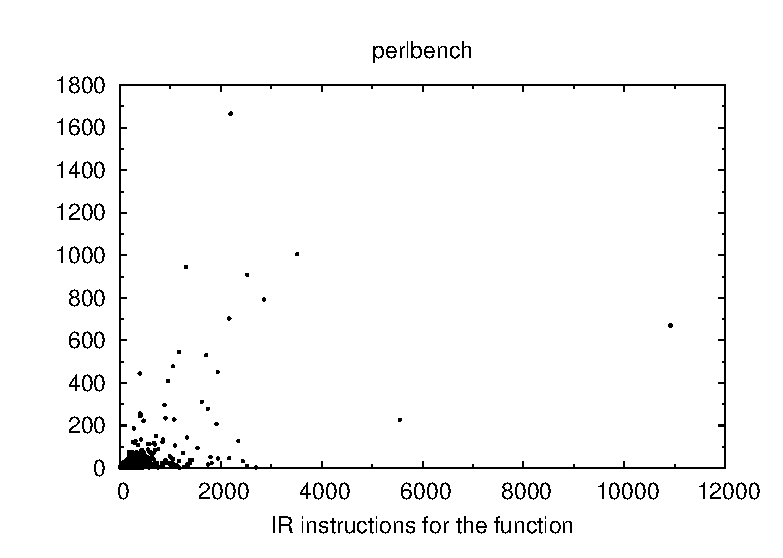
\includegraphics[width=0.45\textwidth]{figures/CS-debug-tot-dead/tot-dead-perlbench-linear.eps}
}
\caption{\protect\label{fig:CS-debug-tot-dead} Scatter plot of the total number of scalar user variables that are endangered by optimizations across program points. The position on the horizontal axis is determined by the number of instructions in each function's unoptimized version. For each selected benchmark we report both a log-log (left) and a linear (right) plot.}
\end{center}
\end{figure}

The log-log plots for \mytt{gcc} may suggest a trend line such that larger functions would typically have a large number of affected variables. However, this trend is less pronounced in \mytt{perlbench}, and nearly absent from \mytt{gobmk}. Linear plots should provide the reader with a better visualization of what happens for larger functions and for functions with a higher total number of affected variables. We can safely conclude that, although larger functions might be more prone to source-level debugging issues, these issues frequently arise for smaller functions as well.

\subsection{Experimental Results}
We have evaluated the ability of \buildcomp\ to correctly reconstruct the source-level expected value for the endangered user variables in the \speccpu\ experiments. For each function, we measured the {\em average recoverability ratio}, defined as the average across all program points corresponding to source-level locations of the ratio between recoverable and endangered user variables for a specific point. Two versions of \reconstruct\ can be useful in this setting: $live_{(e)}$ and $avail$ (\mysection\ref{ss:BC-implementation}).

$live_{(e)}$ can be implemented in debuggers that can evaluate expressions over the current program state, including \gdb\ and LLDB\footnote{As LLDB is tightly coupled with the rest of the LLVM infrastructure, it can also utilize its JIT to run and evaluate arbitrary code. \gdb\ can typically evaluate complex expressions as well.}. In fact, this version of \reconstruct\ needs only to access the live state of the optimized program at the breakpoint.

$avail$ can be integrated in a debugger using {\em invisible} breakpoints to spill a number of non-live available values before they are overwritten. Invisible breakpoints are indeed largely employed in source-level debuggers (e.g., ~\cite{Zellweger83,Wu99,Jaramillo00}). Using spilled values and the current live state, expected values for endangered user variables can be reconstructed as for $live_{(e)}$. Alternatively, in a virtual machine with a JIT compiler and an integrated debugger, the runtime might decide to recompile a function when the user inserts a breakpoint in it, artificially extending the liveness range for the available values that would be needed by \buildcomp.

\begin{figure}[!ht]
\begin{center}
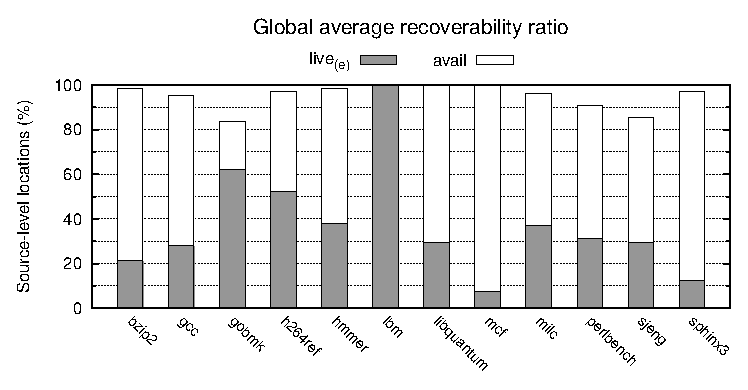
\includegraphics[width=0.8\textwidth]{figures/CS-debug-ratio/CS-debug-ratio.eps}
\caption{\protect\label{fig:CS-debug-ratio} Global average recoverability ratio, defined as weighted average of each function's average recoverability ratio. We used the number of LLVM IR instructions in the unoptimized function version as weight.}
\end{center}
\end{figure}

\noindent \myfigure\ref{fig:CS-debug-ratio} shows for each benchmark the global average recoverability ratio achieved by $live_{(e)}$ and $avail$ on the set of affected functions $F_{end}$. To compute the global average, the average recoverability ratio for each function has been weighted using the number of IR instructions in the unoptimized function as weight. We observe that $avail$ performs particularly well on all benchmarks, with a global ratio higher than $0.95$ for half of the benchmarks, and higher than $0.9$ for $10$ out of $12$ benchmarks. In the worst case (\mytt{gobmk}), we observe a global ratio slightly higher than $0.83$. Results thus suggest that \buildcomp\ can recovery expected values for the vast majority of source-level endangered variables.

\begin{table}[!ht]
\begin{center}
\begin{small}
\begin{adjustbox}{width=0.925\textwidth}
\begin{tabular}{ |c|c|c|c|c|c|>{\centering}p{0.58cm}|c|c|c|c|c|c||c| }
\cline{2-14}
\multicolumn{1}{c|}{} & \rot{bzip2} & \rot{gcc} & \rot{gobmk} & \rot{h264ref} & \rot{hmmer} & \rot{lbm} & \rot{libquantum\hspace{0.5em}} & \rot{mcf} & \rot{milc} & \rot{perlbench} & \rot{sjeng} & \rot{sphinx3} & \rot{Mean} \\
\hline
%$avg$ & 2.29 & 1.99 & 0.38 & 3.48 & 1.95 & 0 & 2.00 & 1.82 & 1.68 & 3.14 & 1.45 & 1.67 & 1.82 \\
%$\sigma$ & 3.20 & 4.51 & 1.23 & 8.09 & 2.33 & 0 & 3.12 & 0.87 & 1.93 & 4.60 & 1.26 & 2.05 & 2.77 \\
%\hline
%C & 12.00 & 77.00 & 12.00 & 88.00 & 9.00 & 0.00 & 10.00 & 3.00 & 8.00 & 32.00 & 5.00 & 11.00 & 22.25 \\
$frac$ & 0.71 & 0.72 & 0.16 & 0.71 & 0.70 & - & 0.67 & 1.00 & 0.76 & 0.66 & 0.77 & 0.72 & 0.69 \\
\hline
$avg$ & 3.24 & 2.77 & 2.31 & 4.90 & 2.79 & - & 3.00 & 1.82 & 2.19 & 4.76 & 1.88 & 2.31 & 2.91 \\ 
\hline
\hline
$\sigma$ & 3.38 & 5.12 & 2.22 & 9.23 & 2.33 & - & 3.46 & 0.87 & 1.94 & 4.94 & 1.12 & 2.08 & 3.34 \\
\hline
\end{tabular} 
\end{adjustbox}
\end{small}
\end{center}
\caption{\label{tab:CS-debug-dead-avail} Available values to preserve when using $avail$. For functions that require to preserve at least one value, we report the fraction $frac$ of $|F_{end}|$ they cumulatively account for, the average number $avg$ of values to preserve across such functions, and the associated standard deviation $\sigma$.
} 
\end{table}

\noindent To estimate how many values should be preserved - through either invisible breakpoints or recompilation - to integrate $avail$ in a debugger, we collected for each function the ``keep'' set of non-live available values to save to support deoptimization across all program points corresponding to source-level locations. We then computed the average and the standard deviation for the size of this set on all functions in $F_{end}$. Figures reported in \mytable\ref{tab:CS-debug-dead-avail} show that typically a third of the functions in $F_{end}$ do not require any values to be preserved. For the remaining functions, on average $2.91$ values need to be preserved, with a peak of $4.90$ observed for \mytt{h264ref}.

Observe that values in the keep set do not necessarily need to be all preserved simultaneously or at all points: indeed, their minimal set can change across function regions. Typically when debugging, what happens is that values are saved using an invisible breakpoint before they are overwritten, and deleted as soon as they are no longer needed~\cite{Jaramillo00}. For the recompilation-based approach, on the other hand, numbers reported in \mytable\ref{tab:CS-debug-dead-avail} should be interpreted as a pessimistic upper-bound for register pressure increase.

\subsection{Comparison with Related Work}
In the previous sections we have seen that our techniques for automatic OSR mapping construction can be useful to restore expected behavior in source-level debuggers. We now discuss the connections of this approach with previous works.

In the debugging literature, we are aware of only one work that supports full source-level debugging. TARDIS~\cite{Barr14} is a time-traveling debugger for managed runtimes that takes snapshots of the program state at a regular basis, and lets the unoptimized code run after a snapshot has been restored to answer queries. Our solution is different in the spirit, as we tackle the problem from the performance-preserving end of the spectrum~\cite{Adl-Tabatabai96thesis}, and in some ways more general, as it can be applied to the debugging of statically compiled languages such as C.

The debugging framework proposed by Wu \etal~\cite{Wu99} selectively takes control of the optimized program execution by inserting breakpoints of four kinds, and then performs a forward recovery process in a complex emulator that executes instructions from the optimized program mimicking their execution order at the source level. Their emulation scheme however cannot report values whose reportability is path-sensitive. The FULLDOC debugger~\cite{Jaramillo00} makes a step further, as it is able to provide truthful behavior for deleted values, and expected behavior for the other values. The authors remark that FULLDOC can be integrated with techniques for reconstructing deleted values, and \buildcomp\ might be an ideal candidate.
%The FULLDOC debugger by Jaramillo \etal~\cite{Jaramillo00}

In his seminal paper~\cite{Hennessy82}, Hennessy presented algorithms for recovering values in locally optimized code, with weaker extensions to globally optimized code. These algorithms, however, can only work with operand values that are user variables coming from memory, as they ignore compiler temporaries or registers. Also because the assumptions made by Hennessy need to be revised due to the advances in compiler and debugging technology~\cite{Copperman93}, these algorithms have not been implemented in real debuggers. Adl-Tabatabai in his PhD thesis~\cite{Adl-Tabatabai96thesis} presents algorithms for recovering values in the presence of local and global optimizations. In particular, the algorithms for global optimizations identifies compiler temporaries introduced by optimizations that alias endangered source variables. This idea is captured by \buildcomp\, which can also use facts recorded during to IR manipulation (\mysection\ref{ss:BC-implementation}) when recursively reconstructing portions of the state for the original program.

%This idea is captured by \buildcomp\, which is able to exploit the OSR mapping information, along with additional facts recorded during IR manipulations (\mysection\ref{ss:BC-implementation}), to reconstruct portions of program state by recursively executing instructions from the original program.